\chapter{Disclosure of Generative AI Use}\label{apd:a}

\section{AI-Assistance}

Generative AI, specifically Gemini models from Google, was extensively used throughout this research. In addition to powering the autonomous agent evaluated in our synthesis benchmark, AI tools assisted in developing experimental test harnesses, analyzing telemetry logs, and drafting initial prose from outlines. All drafted paragraphs were subsequently reviewed, verified, and edited by hand to ensure factual accuracy and academic integrity.

The following agent skills were utilized to support writing and literature verification. Each tool provided automated capabilities within the author's agentic development environment:
\begin{itemize}
	\item \texttt{zotero-cli}: \url{https://github.com/bahayonghang/zotero-cli}
	\item \texttt{thesis-writing-guide}: \url{https://www.skillsdirectory.com/skills/brycewang-stanford-thesis-writing-guide}
\end{itemize}

The \texttt{zotero-cli} skill was used to inspect literature directly from the author's reference library, verifying that source citations accurately represented cited findings. In addition, the \texttt{thesis-writing-guide} skill provided structured feedback on chapter organization, academic tone, and university formatting compliance.

\section{AI-Generated Artifacts}

The student onboarding guide presented below (\texttt{nix\_installation\_guide.pdf}) was generated with AI assistance to support the onboarding evaluations. It provides step-by-step instructions for installing the Nix package manager and activating coursework development shells via \texttt{nix develop}:

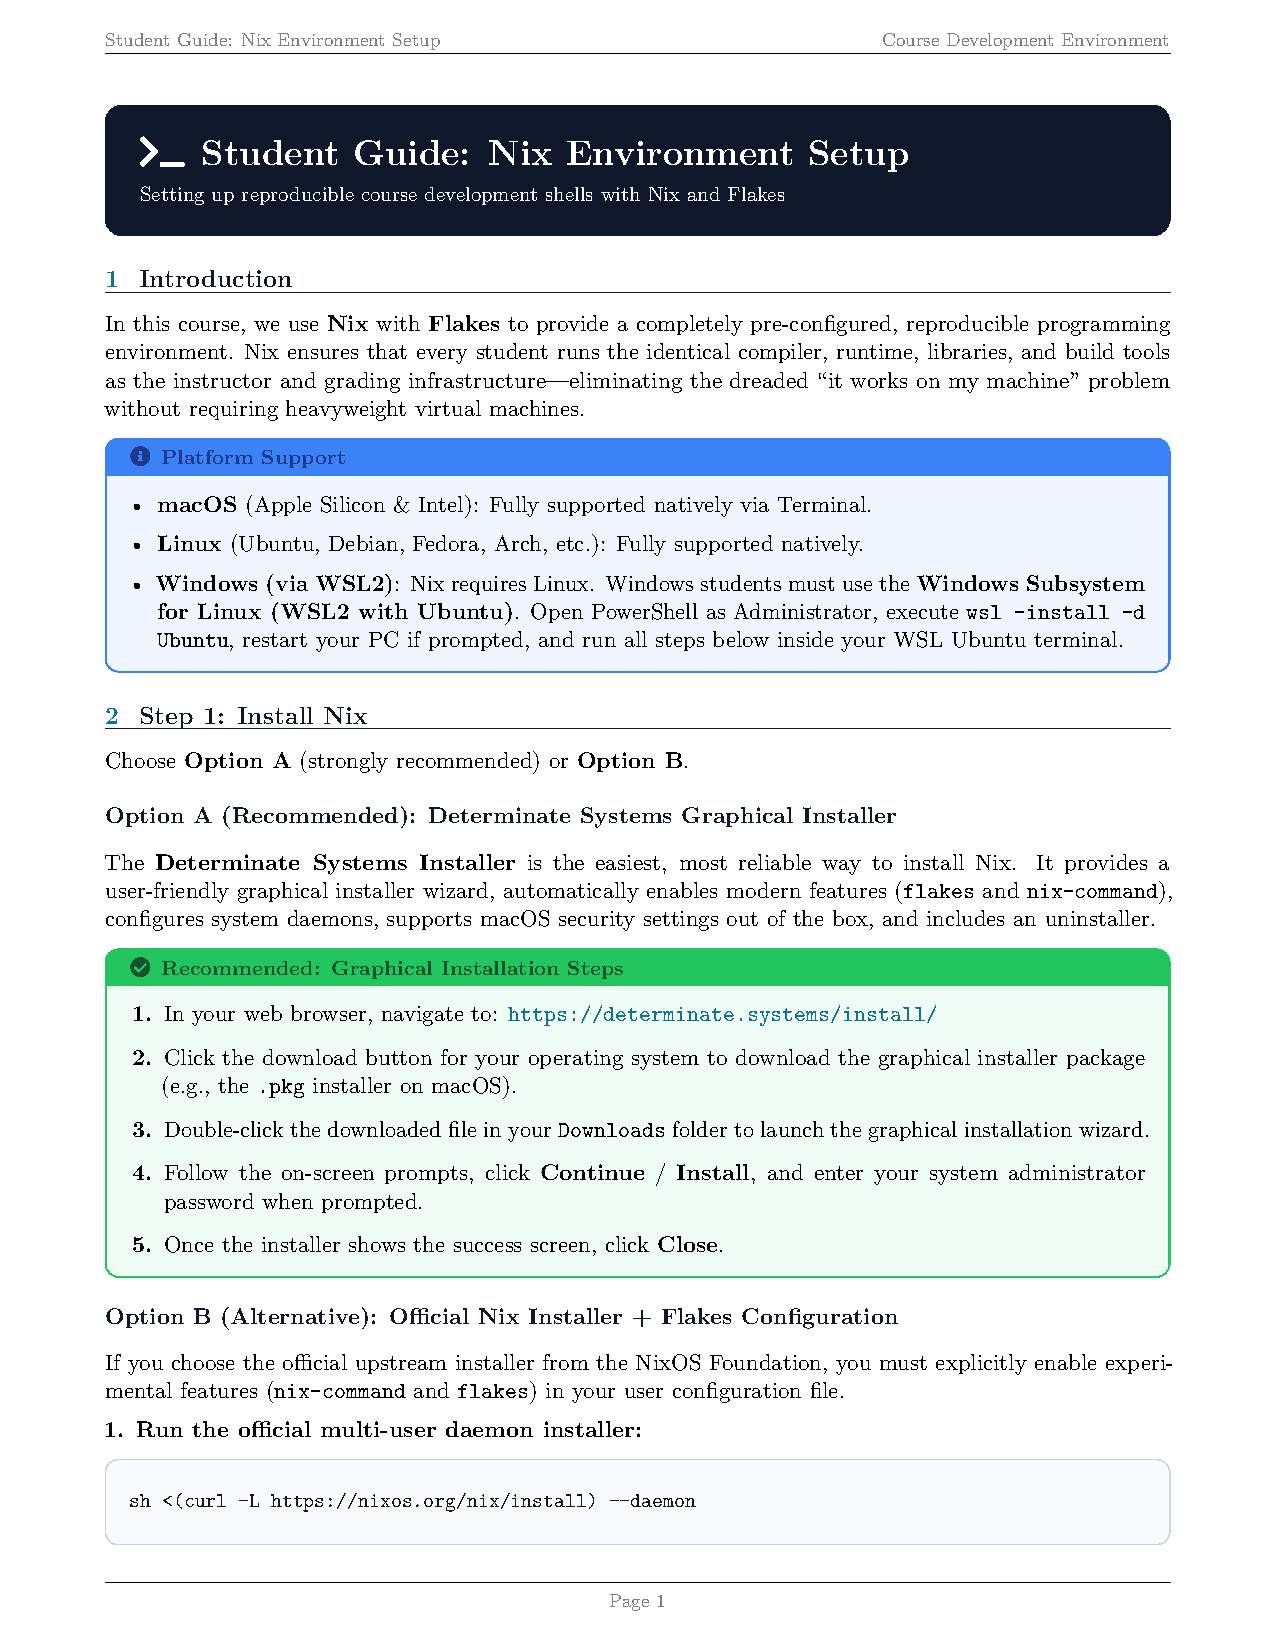
\includepdf[pages=-,scale=0.82,pagecommand={\thispagestyle{myheadings}}]{Figures/nix_installation_guide.pdf}

\subsection{AI-Generated Input for RQ1}

The synthetic natural language benchmark instructions (Listing~\ref{lst:nl-instruction-inputs}) were generated with AI assistance to evaluate RQ1 across the Software Development and Data Science curriculum tracks. These prompts are grounded in the author's practical experience across university computer science courses, establishing realistic requirement statements paired with expected CLI dependency assertions.

\begin{lstlisting}[caption={Natural Language Instruction Benchmark Inputs}, label={lst:nl-instruction-inputs}]
{"track":"computer science","instruction":"Install Java JDK 17 (includes the JRE). Set JAVA_HOME to the JDK install directory (not a separate JRE folder) and add $JAVA_HOME/bin to your PATH. Install Visual Studio Code, then install the Java extension pack (Language Support for Java by Red Hat, Debugger for Java, Java Test Runner, Maven for Java). Restart VS Code and verify with `java -version` and `javac -version`.","dependency_list":["java","javac","code"]}
{"track":"computer science","instruction":"Install the Flutter SDK and ensure `flutter` is on your PATH. Run `flutter doctor` and follow the prompts to install/fix any missing platform toolchains it reports.","dependency_list":["flutter","dart"]}

{"track":"computer science","instruction":"Install Python 3.12 and the `uv` package manager. In your project directory, run `uv add` for the following packages: flask and flask-restful, then `uv sync`. Verify with `python3 --version` and `uv --version`.","dependency_list":["python3","uv"]}
{"track":"computer science","instruction":"Install GCC (C/C++) and build tools. Verify with `gcc --version`, `g++ --version`, `cmake --version`, and `make --version`, then build the project using the provided build instructions.","dependency_list":["gcc","g++","cmake","make"]}
{"track":"computer science","instruction":"Install Clang (C/C++) and build tools. Verify with `clang --version`, `clang++ --version`, `cmake --version`, and `make --version`, then build the project using the provided build instructions.","dependency_list":["clang","clang++","cmake","make"]}
{"track":"computer science","instruction":"Install Node.js (LTS) so you have `node` and `npm`. Verify with `node --version` and `npm --version`, then run `npm install` in the project directory.","dependency_list":["node","npm"]}
{"track":"computer science","instruction":"Install Rust using rustup, then ensure `rustc` and `cargo` are available. Verify with `rustc --version` and `cargo --version`, then run `cargo build`.","dependency_list":["rustup","rustc","cargo"]}
{"track":"computer science","instruction":"Install Go and confirm the `go` command is available. Verify with `go version`, then run `go test ./...` in the project directory.","dependency_list":["go"]}
{"track":"computer science","instruction":"Install the .NET SDK (not just the runtime). Verify with `dotnet --info`, then run `dotnet restore` and `dotnet build`.","dependency_list":["dotnet"]}
{"track":"computer science","instruction":"Install Ruby and Bundler. Verify with `ruby --version` and `bundle --version`, then run `bundle install`.","dependency_list":["ruby","bundle"]}

{"track":"data science","instruction":"Install R (latest stable). Ensure the `R` executable is on your PATH, then verify with `R --version` and starting an interactive session with `R`.","dependency_list":["R"]}
{"track":"data science","instruction":"Install RStudio Desktop and launch it once to confirm it detects your R installation. If it does not, configure RStudio to point to the installed R version in its settings.","dependency_list":["R","rstudio"]}
{"track":"data science","instruction":"Install MySQL Server, start the database service, and set a root password. Verify by connecting with `mysql -u root -p` and running `SELECT VERSION();`.","dependency_list":["mysqld","mysql"]}
{"track":"data science","instruction":"Install MySQL Workbench (GUI client). Create a new connection to your local MySQL server and test the connection using the credentials you set.","dependency_list":["mysql-workbench","mysqld","mysql"]}
\end{lstlisting}